\documentclass[10pt, compress]{beamer}
\usetheme{m}
\usepackage{booktabs}
\usepackage[russian]{babel}
\usepackage[scale=2]{ccicons}
\usepackage{minted}
\usepackage[plain]{algorithm}
\usepackage{algorithmicx}
\usemintedstyle{trac}
\usepackage{varwidth}
\usepackage{xspace}
\usepackage{xcolor}
\usepackage{algpseudocode}
\algnewcommand\algorithmicand{\textbf{and}\xspace}
\algnewcommand\algorithmicor{\textbf{or}\xspace}
\algnewcommand\algorithmicnot{\textbf{not}\xspace}
\algnewcommand\algorithmictrue{\textbf{true}}
\algnewcommand\algorithmicfalse{\textbf{false}}
\algtext*{EndWhile} % Remove "end while" text
\algtext*{EndIf} % Remove "end if" text
\algtext*{EndFor} % Remove "end for" text
\algtext*{EndProcedure} % Remove "end for" text
%---------------------------------------------------------------------------------------

\title{Параллельные алгоритмы поиска кратчайших путей на графах}
\subtitle{}
\date{\today}
\author{Выполнил: Ткаченко Г.C. \\ Руководитель: Корнеев Г.А.}
\institute{Университет ИТМО}

\begin{document}

\maketitle

\section{Проблема и задача}
\begin{frame}[fragile]
  \frametitle{Решаемая проблема}

\begin{itemize}
	\item Недостаточное разнообразие параллельных алгоритмов для поиска кратчайших путей

    \item Низкая производительность отдельных алгоритмов на специфичных графах    
  \end{itemize}
\end{frame}

\begin{frame}[fragile]
  \frametitle{Постановка задачи}
\begin{itemize}
    \item Эффективное применение алгоритмов поиска кратчайшего пути на \textbf{многопроцессорных} архитектурах
    \item Разработка алгоритмов для поиска пути от одной вершины до всех (\textbf{one-to-many})
    \item Разработка алгоритмов для поиска пути кратчайшего расстояния между каждой парой вершин (\textbf{many-to-many})
  \end{itemize}
\end{frame}

\section{Задача one-to-many}

\begin{frame}[fragile]
  \frametitle{Обзор решений}
\begin{itemize}
    \item \textbf{Алгоритм Беллмана-Форда}
    \begin{itemize}
    	\item Классический
    	\item На основе обхода в ширину
	\end{itemize}	   
	\item Алгоритм Дейкстры
    \item Алгоритмы A*
    \item Алгоритмы D*
  \end{itemize}
\end{frame}

\begin{frame}[fragile]
  \frametitle{Параллельный Беллман-Форд}
  Три подхода
  \begin{itemize}
    \item Параллелизация по ребрам вершины
    \item Параллелизация по всем ребрам
    \item Использование параллельного обхода в ширину
  \end{itemize}
\end{frame}

\begin{frame}[fragile]
  \frametitle{Параллелизация по ребрам вершины}
  {\vspace{-2em}\begin{center}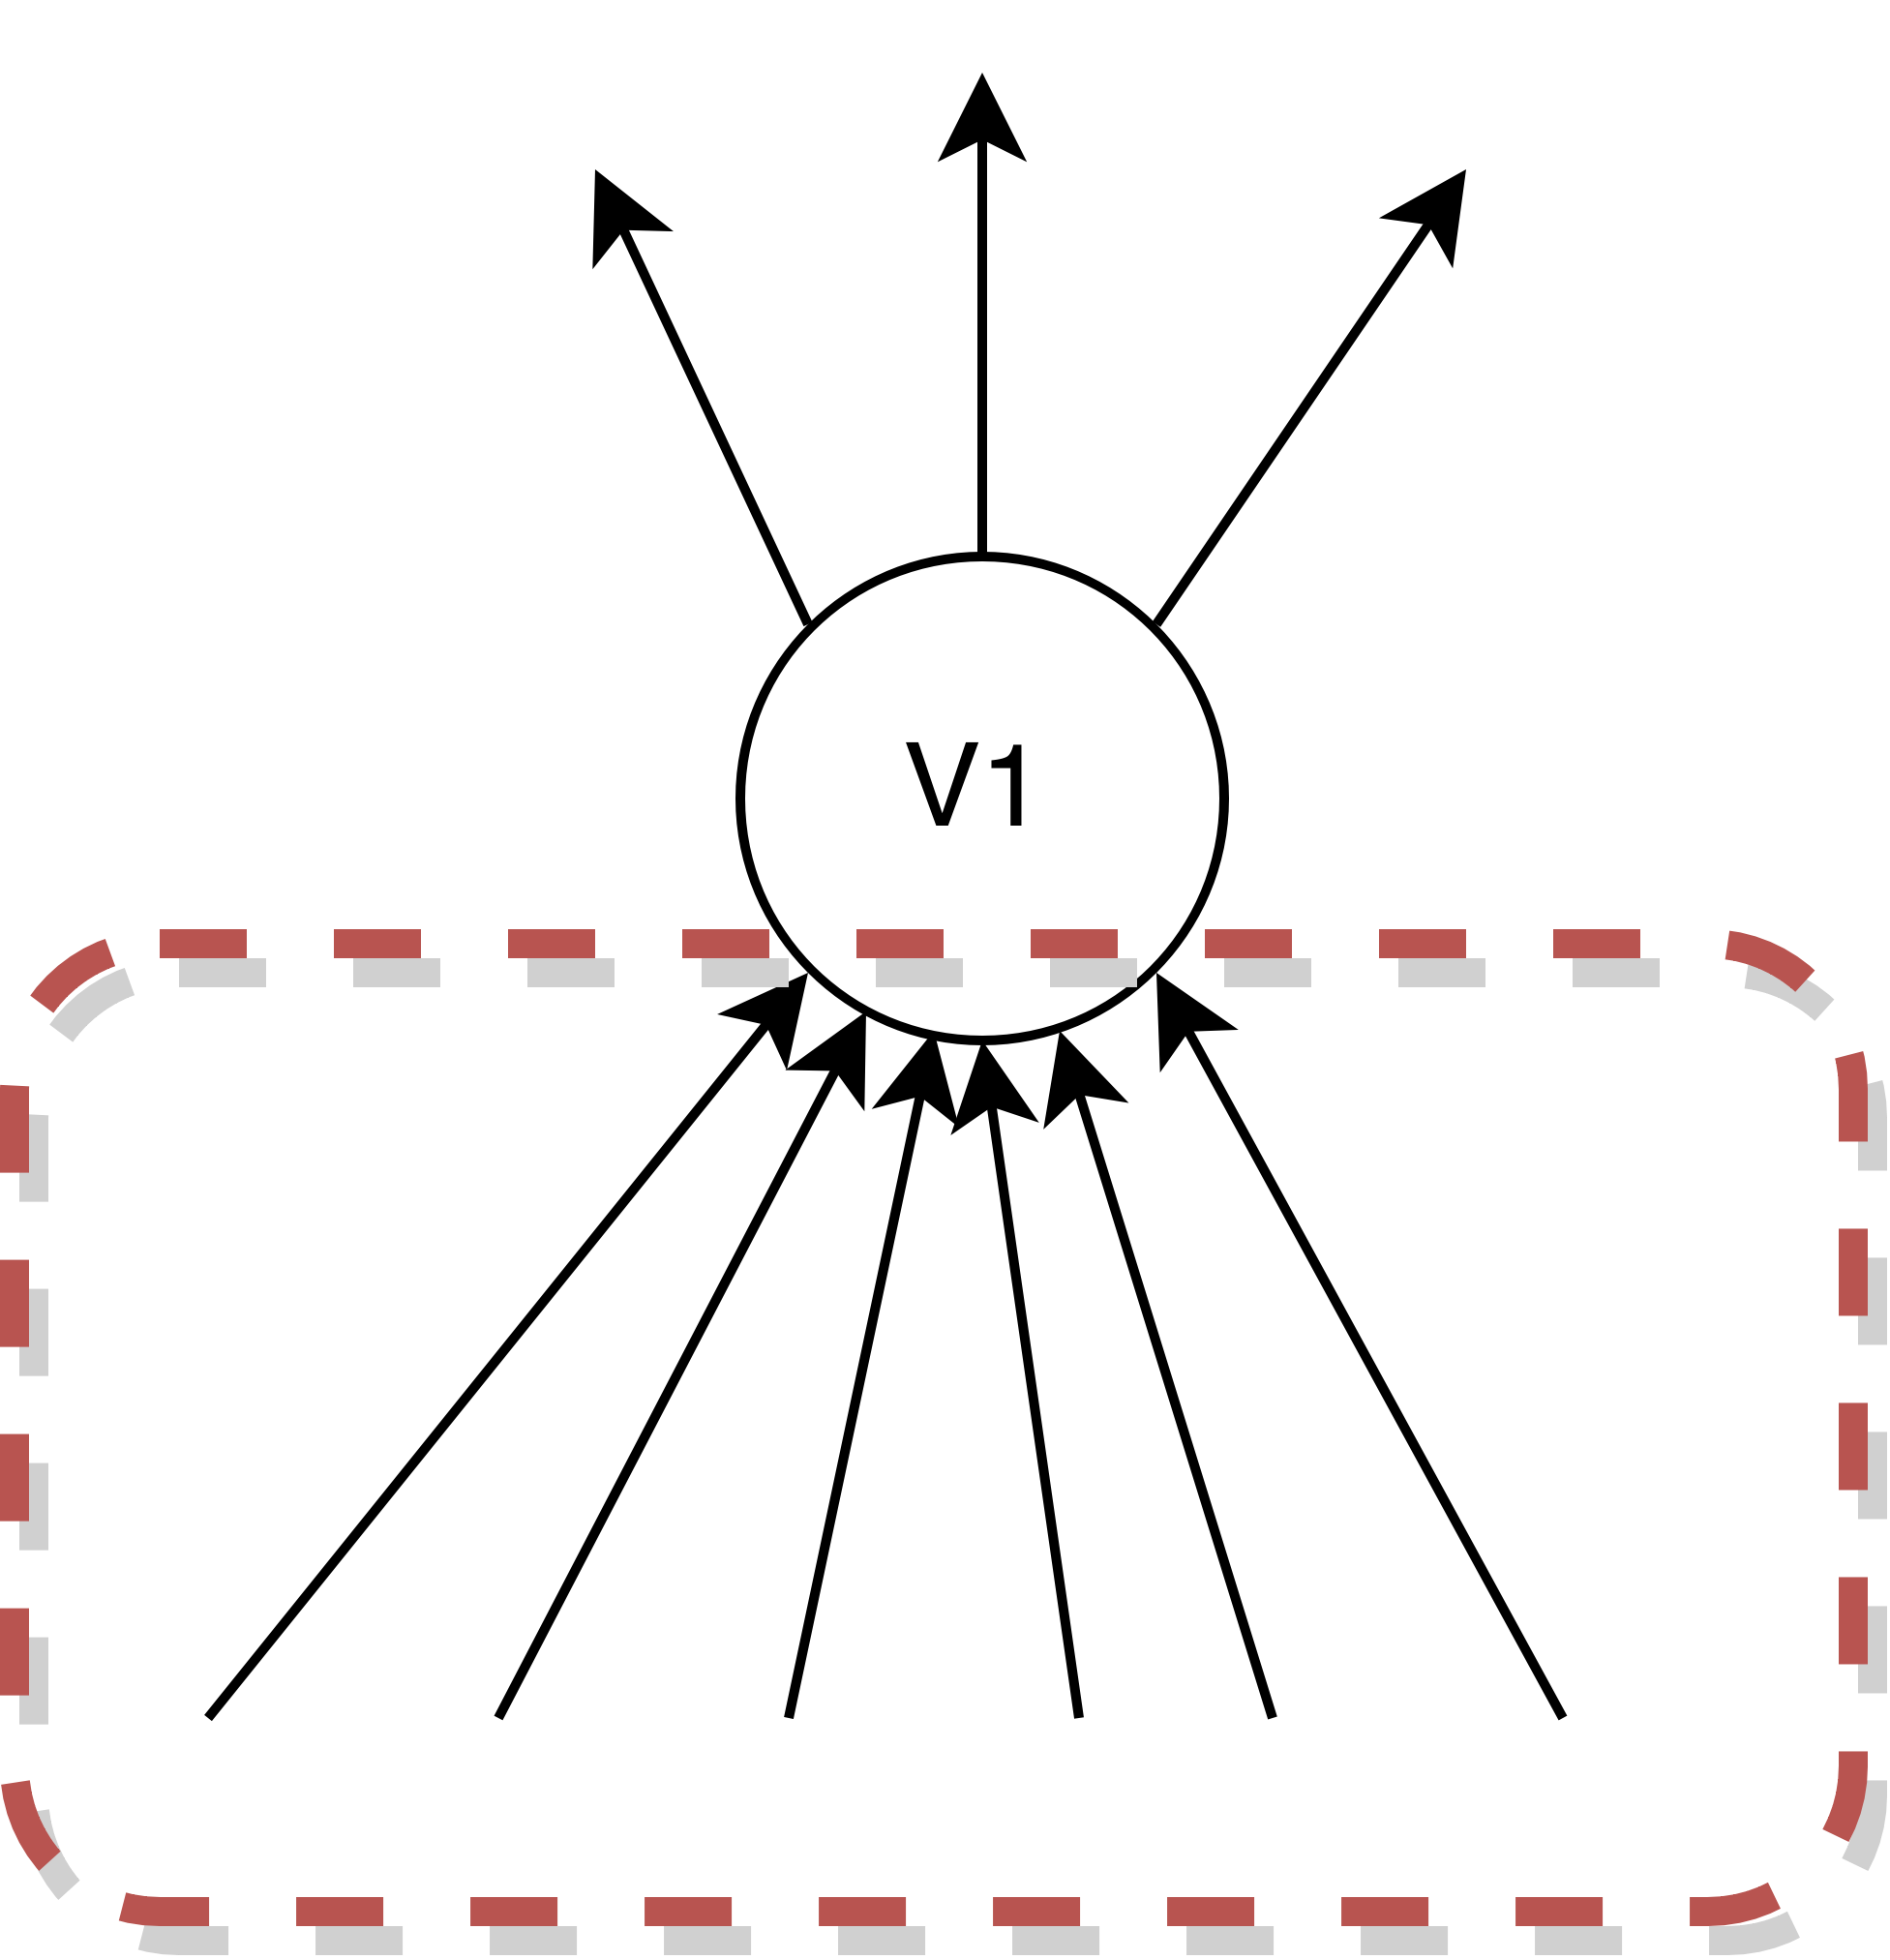
\includegraphics[height=0.75\textheight]{images/bf_par_1.png}\end{center}}
\end{frame}

\begin{frame}[fragile]
  \frametitle{Параллелизация по всем ребрам}
  {\vspace{-2em}\begin{center}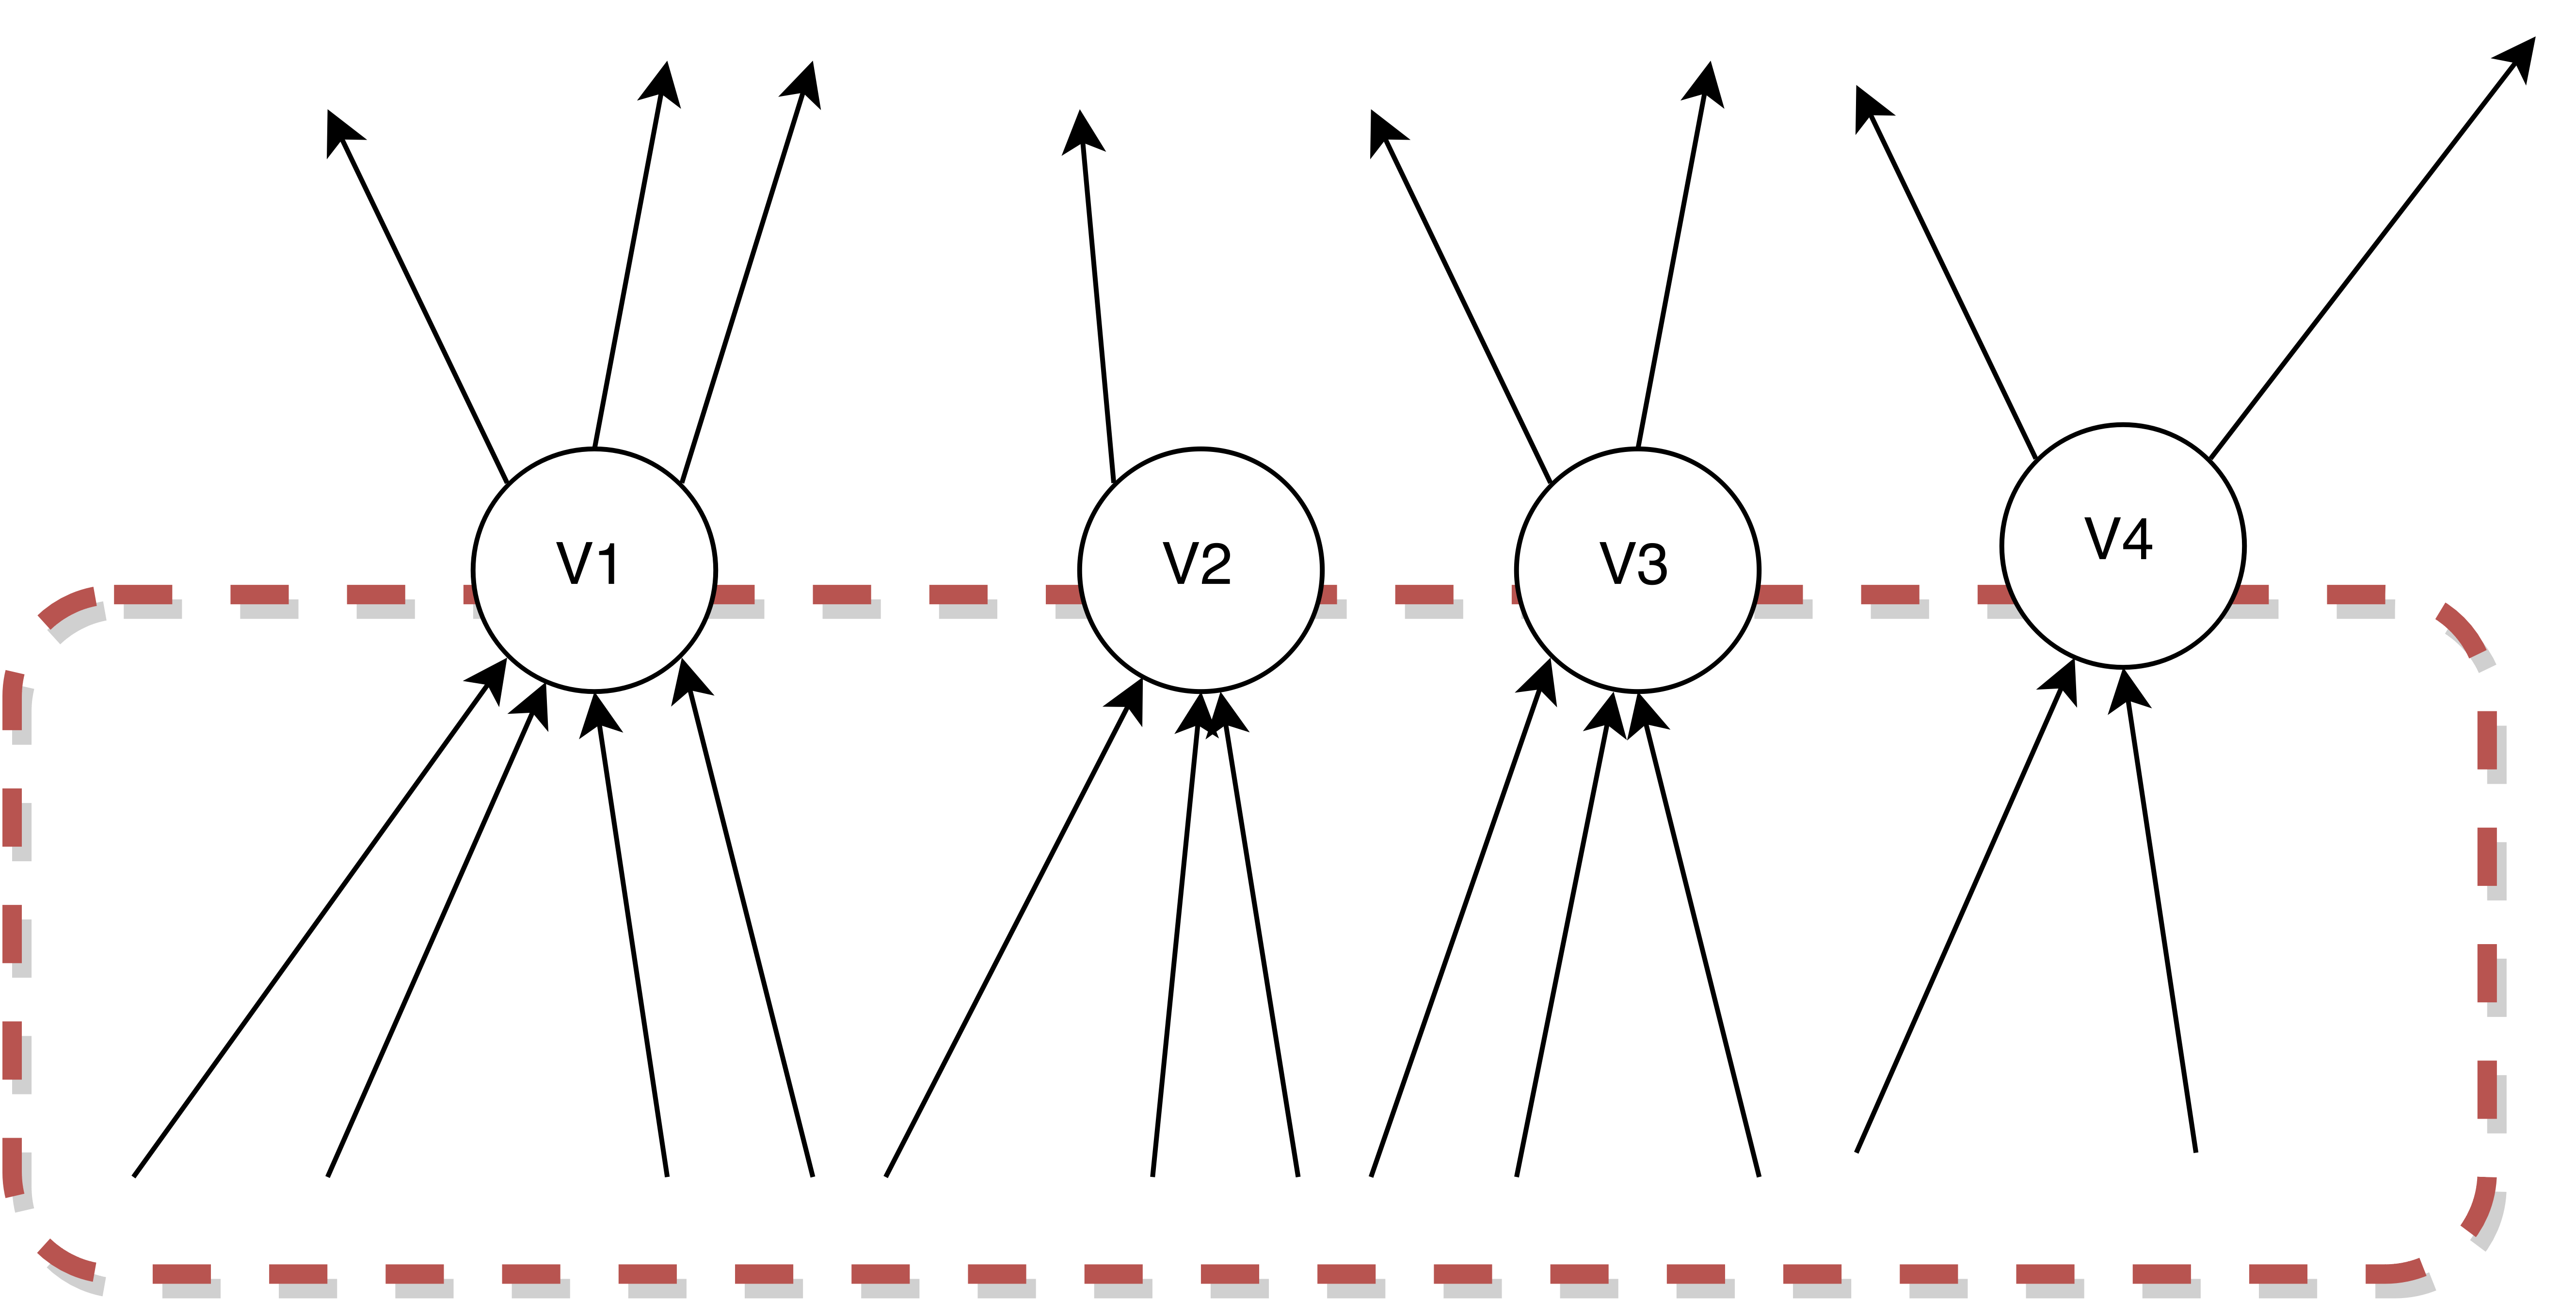
\includegraphics[width=\textwidth]{images/bf_par_2_1.png}\end{center}}
\end{frame}
\begin{frame}[fragile]
  \frametitle{Параллелизация по всем ребрам}
  {\vspace{-2em}\begin{center}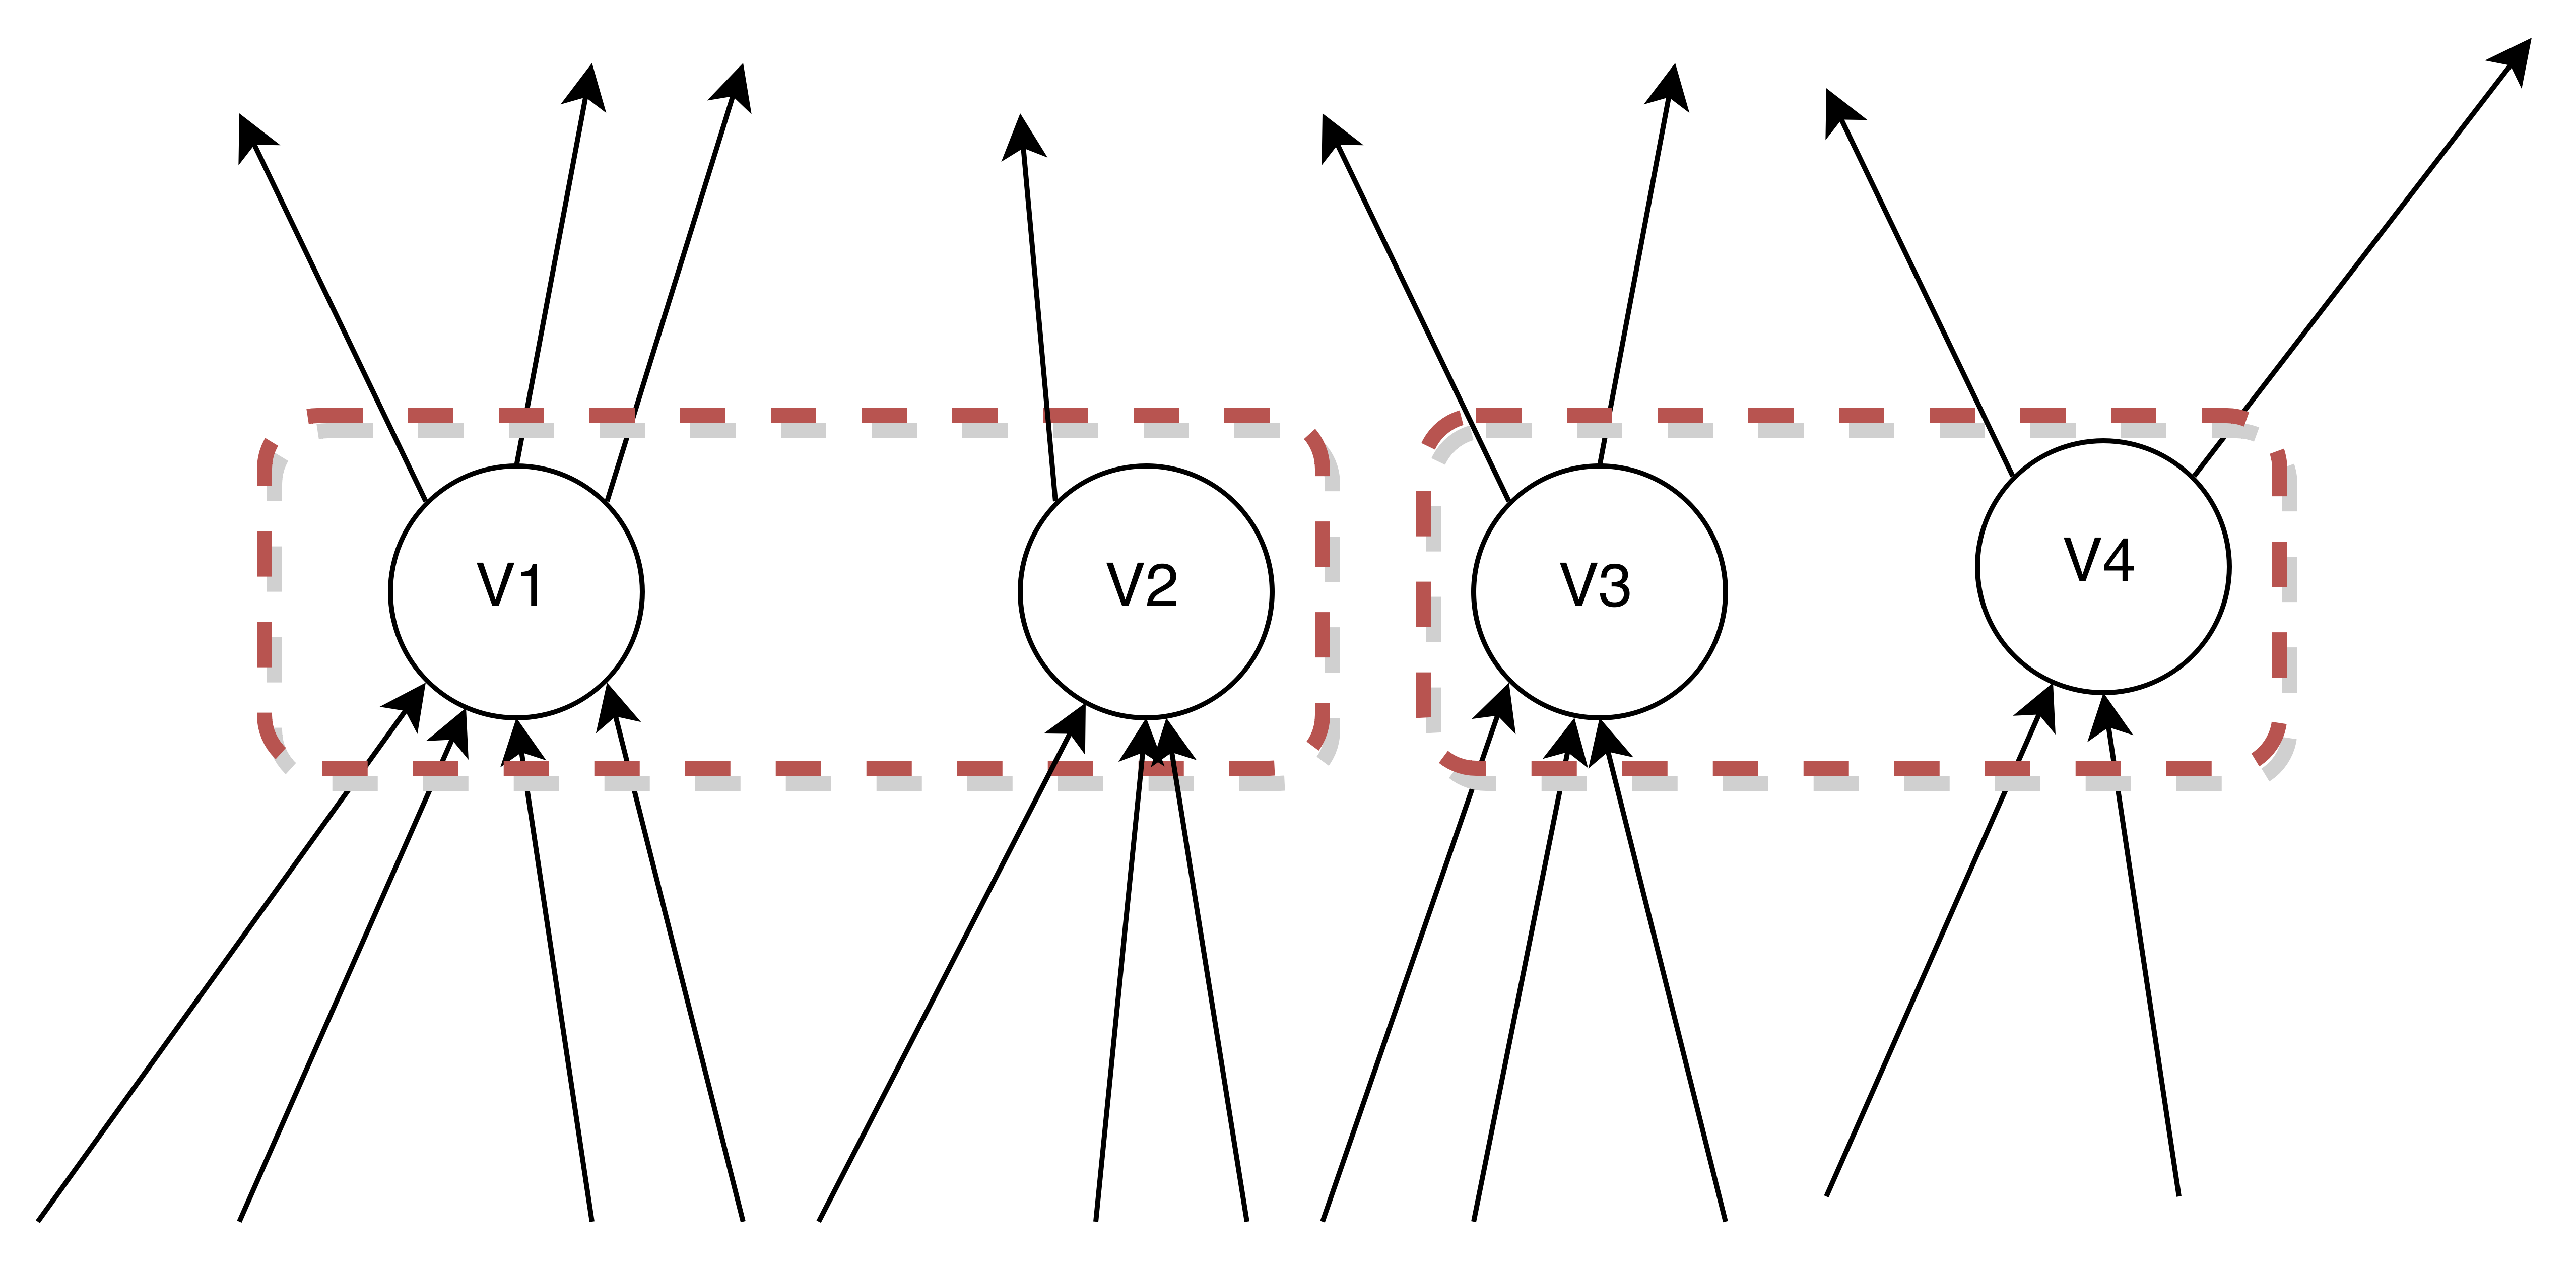
\includegraphics[width=\textwidth]{images/bf_par_2_2.png}\end{center}}
\end{frame}

\begin{frame}[fragile]
  \frametitle{Использование параллельного обхода в ширину}
  {\vspace{-2em}\begin{center}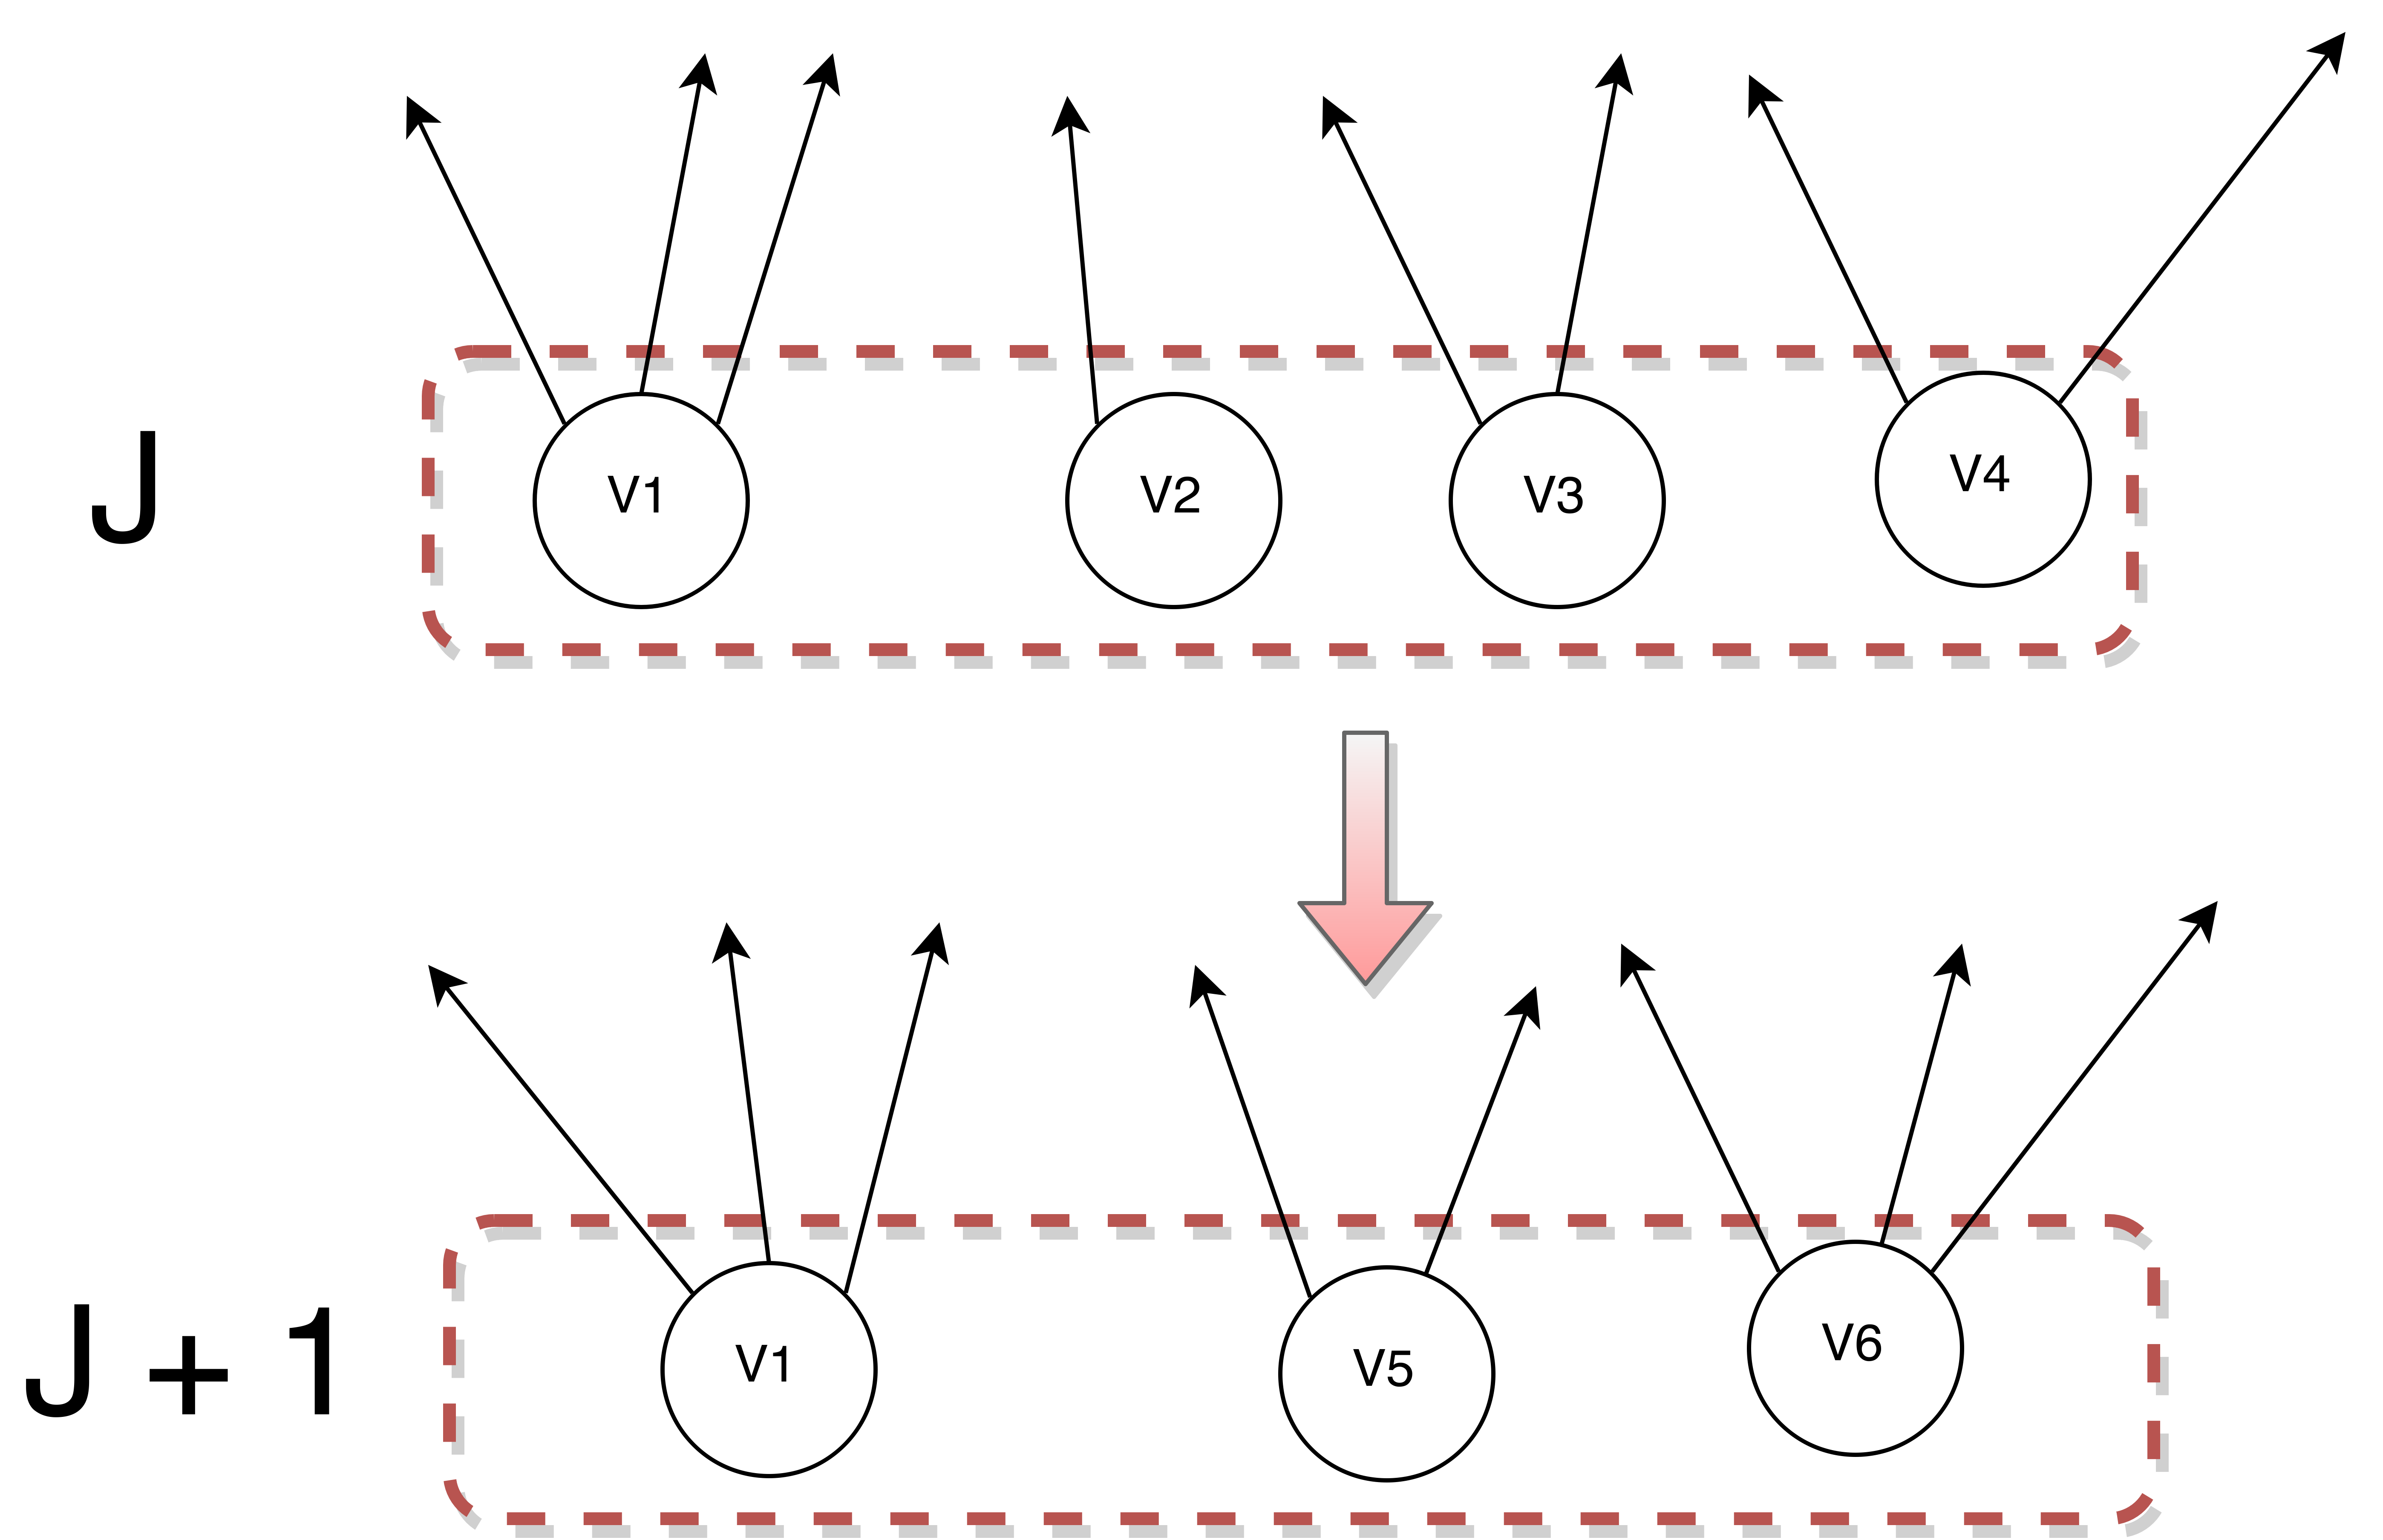
\includegraphics[width=\textwidth]{images/bf_par_3.png}\end{center}}
\end{frame}

\section{Задача many-to-many}


\begin{frame}[fragile]
  \frametitle{Алгоритм Флойда}
  \begin{itemize}
    \item В некоторых случаях классический алгоритм оказывается медленнее наивных алгоритмов
    \item Для каждой вершины можно использовать любой алгоритм поиска кратчайшего пути
  \end{itemize}
\end{frame}


\begin{frame}[fragile]
  \frametitle{Наивная параллельная версия}
\begin{algorithm}[H]
\begin{algorithmic}[1]
\Procedure{AllPairsPar1}{$G$}
\State \textbf{return} {\Call {HandleVertices}{$G, 0, |G.vertices|$}}
\EndProcedure
\State
\Procedure{HandleVertices}{$G, startV, endV$}

\If {$endV - startV < threshold$} 
	\State run Bellman-Ford for $[startV, endV)$
\Else	
	\State $midV \gets (startV + endV) / 2$ 
	\State \begin{varwidth}[t]{\linewidth}fork2(\par
        \hskip\algorithmicindent {\Call {HandleVertices}{$G, startV, midV$}},\par
        \hskip\algorithmicindent {\Call {HandleVertices}{$G, midV, endV$}});
      \end{varwidth}
	
\EndIf

\EndProcedure
\end{algorithmic}
\end{algorithm}
\end{frame}

\begin{frame}[fragile]
  \frametitle{Алгоритм для социальных графов}
  \begin{itemize}
    \item Основан на теории \textbf{«Шести рукопожатий»}
    \item Работает не неориентированных невзвешенных социальных графах
    \item Использует идею динамического программирования
  \end{itemize}
\end{frame}

\begin{frame}[fragile]
  \frametitle{Идея}
    {\vspace{-2em}\begin{center}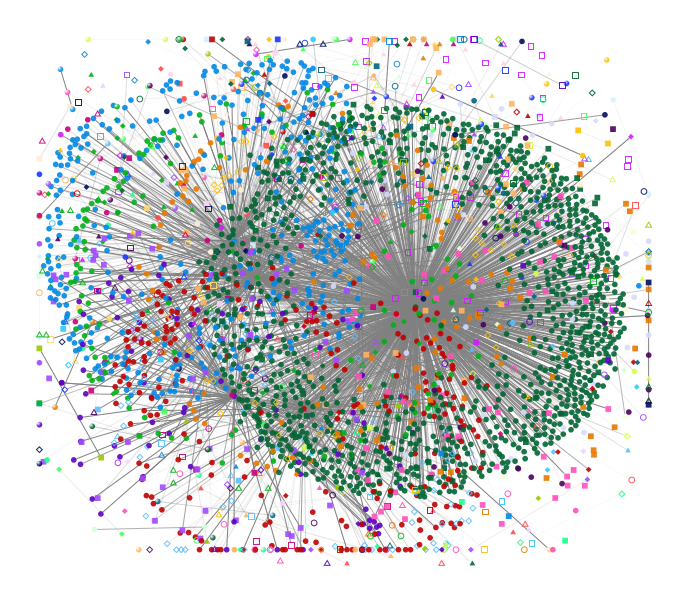
\includegraphics[width=0.8\textwidth,height=0.8\textheight]{images/floyd_social_1.png}\end{center}}

\end{frame}

\begin{frame}[fragile]
  \frametitle{Идея}
    {\vspace{-2em}\begin{center}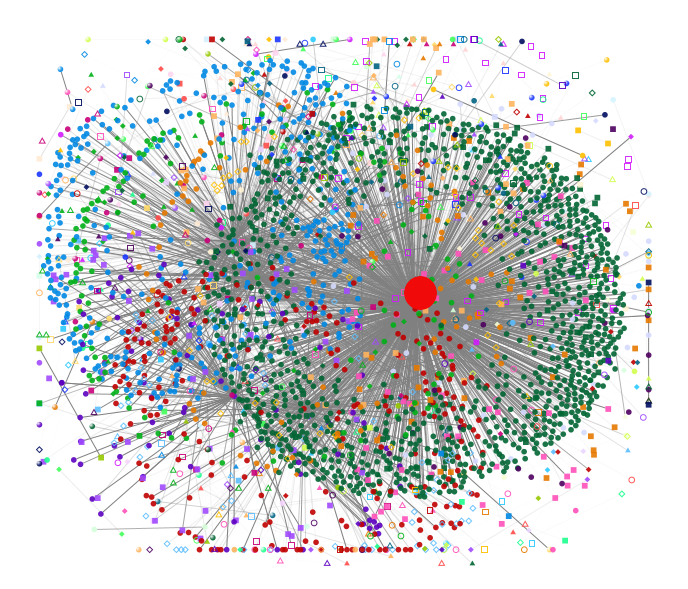
\includegraphics[width=0.8\textwidth,height=0.8\textheight]{images/floyd_social_2.png}\end{center}}

\end{frame}

\begin{frame}[fragile]
  \frametitle{Идея}
    {\vspace{-2em}\begin{center}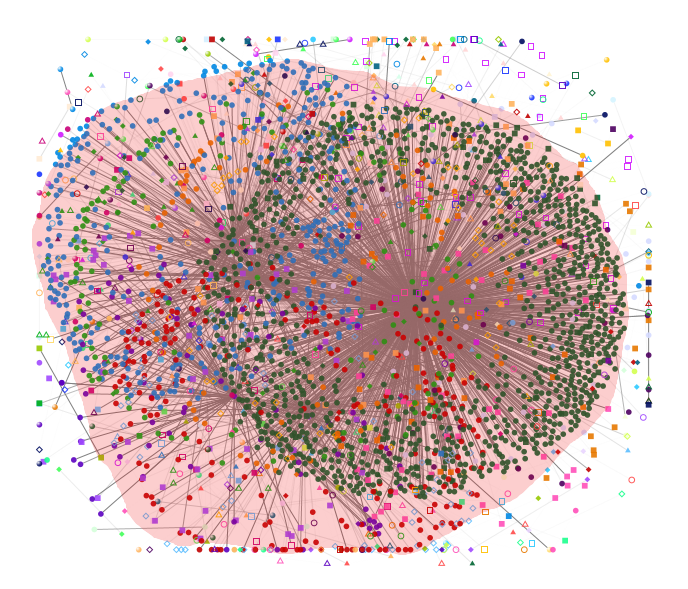
\includegraphics[width=0.8\textwidth,height=0.8\textheight]{images/floyd_social_3.png}\end{center}}

\end{frame}

\begin{frame}[fragile]
  \frametitle{Идея}
    {\vspace{-2em}\begin{center}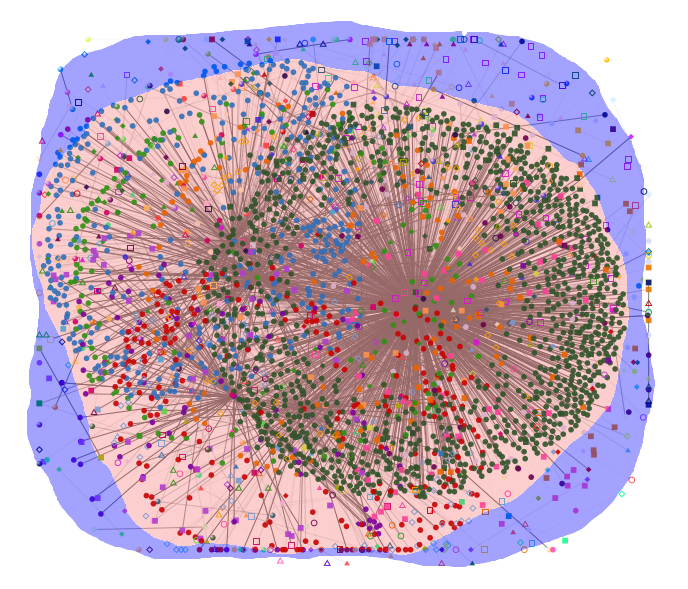
\includegraphics[width=0.8\textwidth,height=0.8\textheight]{images/floyd_social_4.png}\end{center}}

\end{frame}

\begin{frame}[fragile]
  \frametitle{Динамика для большего множества}
    \begin{itemize}
    	\item Основана на \textbf{битовых векторах}
		\item mask[v][i] --- множество вершин $U$, что $\forall u \in U, \ p(u, v) = i$
		\item calc[v][i] $ \ \ $--- множество вершин $U$, что  $\forall u \in U, \ p(u, v) < i$
		\item \textbf{$O(V)$} битовых векторов
	\end{itemize}
	
	\begin{equation}
mask[v][i] = \neg calc[v][i - 1] \wedge \bigvee_{\exists (u, v) \in E} mask[u][i - 1] 
\end{equation}

\begin{equation}
calc[v][i] = calc[v][i - 1] \vee mask[v][i]
\end{equation}

\end{frame}

\section{Результаты}

\begin{frame}[fragile]
  \frametitle{Технологии}
\begin{itemize}
    \item C++11
    \item PASL (Parallel Algorithm Scheduling Library)
    \item 40-core Intel machine (with hyper-threading) 
  \end{itemize}
\end{frame}


\definecolor{cssgreen}{rgb}{0.0, 0.5, 0.0}

\begin{frame}[fragile]
  \frametitle{Сравнение параллельных версий Беллмана-Форда}
\begin{table}
\centering
\begin{tabular}{l|ccc|cc|cc}  
Идея алгоритма& \multicolumn{3}{c}{Полный} & \multicolumn{2}{c}{Дерево} & \multicolumn{2}{c}{Решетка} \\
& TS & + & +- & 0.5 & 1 & + & +- \\
\hline\hline
Ребра вершины & \textcolor{cssgreen}{2.43} & 4.65 & $\infty$ & 116.31 & 9.04 & 5.49 & 13.40\\  
Все ребра & 5.17 & \textcolor{cssgreen}{0.18} & \textcolor{cssgreen}{10.84} & 3.59 & 3.08 & 5.92 & 7.10  \\
Обход в ширину & 44.63 & 0.37 & 23.55 & \textcolor{cssgreen}{0.44} & \textcolor{cssgreen}{0.31} & \textcolor{cssgreen}{4.42} & \textcolor{cssgreen}{0.58} \\
Ligra & 49.13 & 0.30 & 26.11 & 0.55 & 0.50 & 8.15 & 1.21 \\
\end{tabular}
\label{graph_description}
\end{table}


\begin{table}
\centering
\begin{tabular}{l|ccc|ccc}  
Идея алгоритма& \multicolumn{3}{c}{Разреженный} & \multicolumn{3}{c}{Плотный}\\
& 0.5+  & 0.5+- & 0.96+ & 0.5+ & 0.5+- & 0.96+\\
\hline\hline
Ребра вершины & $\infty$ & $\infty$ & 24.35 & $\infty$ & $\infty$ & 5.01 \\  
Все ребра & 2.77 & \textcolor{cssgreen}{14.68} & 2.42 & \textcolor{cssgreen}{0.48}  & \textcolor{cssgreen}{6.38}  & \textcolor{cssgreen}{0.46} \\
Обход в ширину & 0.59 & 22.59 & \textcolor{cssgreen}{0.48}  & 0.60  & 10.25 & 0.71 \\
Ligra & \textcolor{cssgreen}{0.58} & 25.19 & 0.54 & 1.12  & 14.15 & 1.20 \\
\end{tabular}
\label{graph_description}
\end{table}

\end{frame}


\begin{frame}[fragile]
  \frametitle{Расстояние между каждой парой вершин социального графа}

\begin{table}
\centering

\begin{tabular}{l|c|c}  
Алгоритм & Twitter & Slashdot\\
\hline\hline
Стандартная параллельная версия & 427.217 & 254.567 \\  
Алгоритм для социальных графов & \textcolor{cssgreen}{191.232} & \textcolor{cssgreen}{169.393}  \\
\hline
\end{tabular}

\caption{Сравнение алгоритмов}
\label {table:algo_floyd_comparison}
\end{table}
  
\end{frame}


\begin{frame}[fragile]
  \frametitle{Итого}
  \begin{itemize}
    \item Разработаны параллельные версии Беллмана-Форда 
    \item Разработан алгоритм для социальных графов
    \item Алгоритмы показали высокую эффективность на практике
    \item Исследованы области применимости алгоритмов
  \end{itemize}
\end{frame}

\end{document}
